\documentclass{standalone}
% preamble: usepackage, etc.
\begin{document}
	
\chapter{代码实现及实验}
在本章,我们将给出基于强化学习的路径规划问题的算法实现,以及实验结果展示。首先我们介绍为实现该算法,我们设计并开发了一个基于 Python 的强化学习框架,其包括了 Q-leanring 等多个方法,同时我们实现了多个场景下的地图环境,然后给出我们的实验设计和参数的设置。其次我们给出实验的结果,以及对结果的简要分析。
\section{基于面向对象设计的代码实现}
在代码实现上,我们基于 Python语言实现了基于面向对象设计思想的代码框架,以期望代码能够具有较高的鲁棒性和重用性和灵活性。\par
首先在类的设计上,我们将智能体抽象为代码中的 Agent 类,环境抽象为Environment 类,两者都是一个抽象类(Abstract Class),其次,我们将任何一种算法抽象为 Model 类(同样为抽象类),通过分离智能体和模型类,可以使得智能体方便载入各种不同的算法,并保持自身行为方式不改变,这使用了设计模式中的典型的策略模式(Strategy Pattern)。同时我们设计了Config 类用于托管各个模块的配置文件,超参数等,这些参数在实验开始时通过本地的文件加载进来,这使得我们解除了所有的硬编码(Hard Code),使得对实验的调参工作只需要更改配置文件即可实现,从而变得相对容易和灵活。同时,我们设计了一个 Sampler 的类。它将托管智能体与环境的交互过程,即采样过程,这使得我们能通过实现不同的 Sampler 类,轻松的更改对采样过程的控制。整个代码的UML图如下:
\begin{figure}
	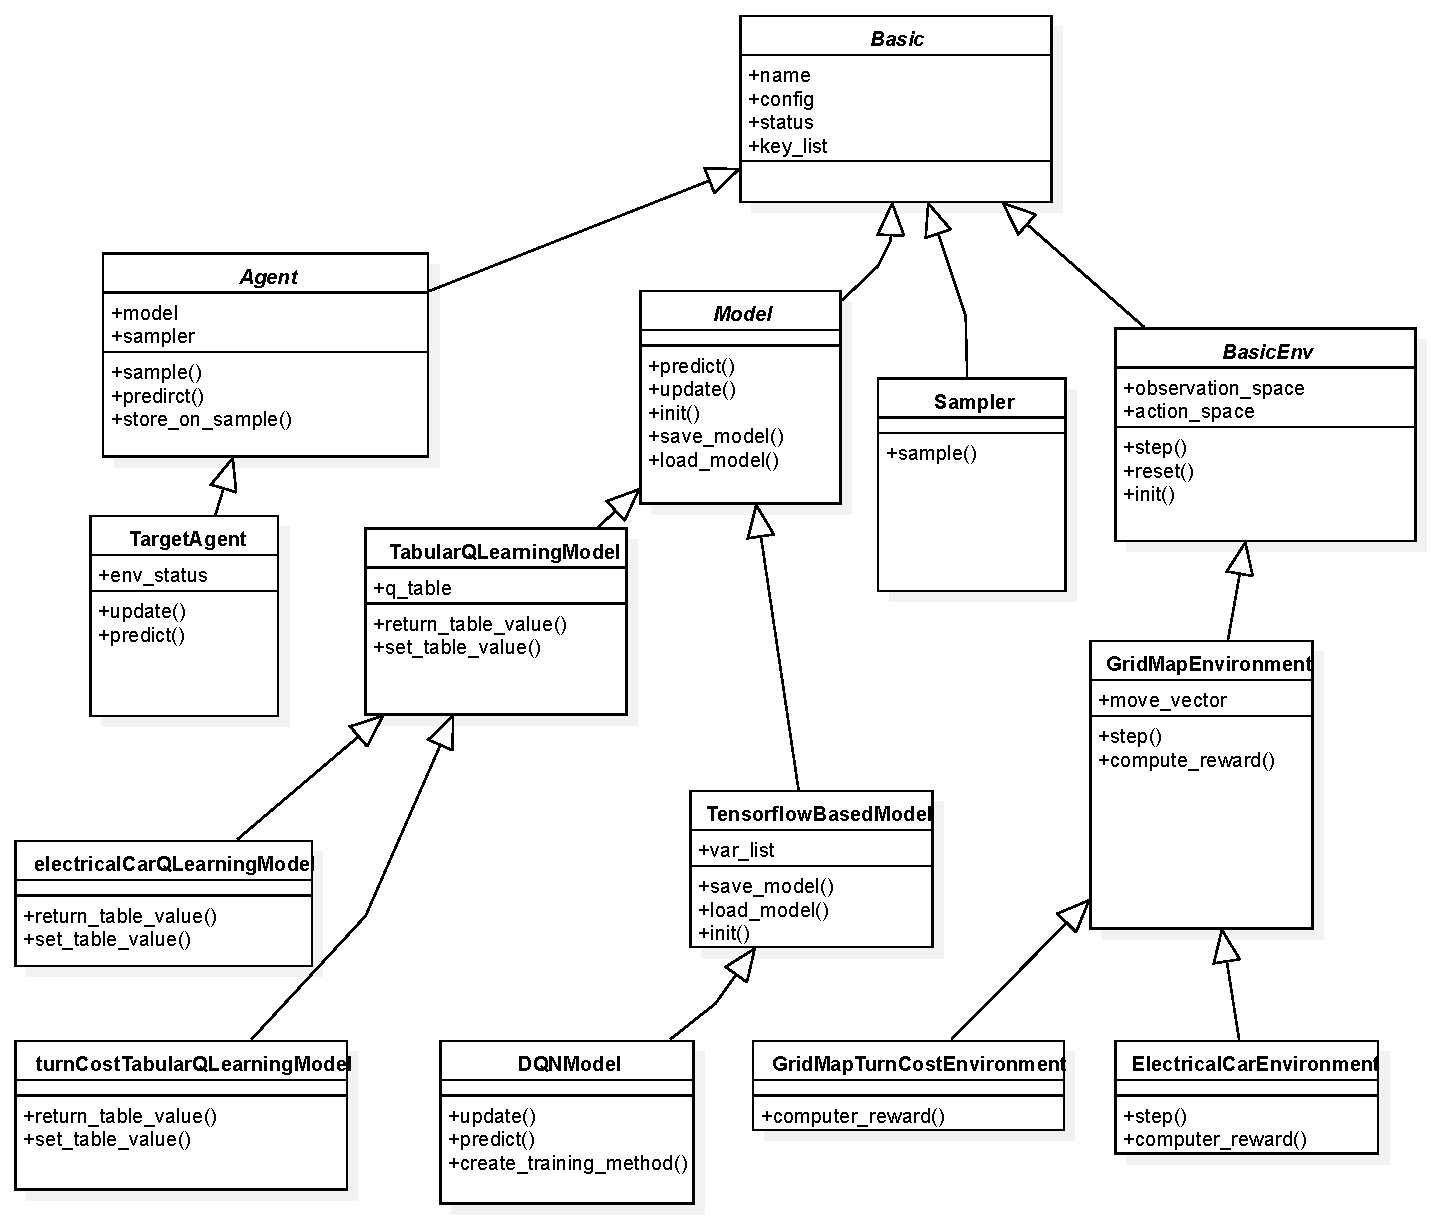
\includegraphics[width=12.0cm]{pic/6-1.pdf}
	\caption{代码实现 UML 图}
	\label{6-1}
\end{figure}

对于实验过程的监视和结果的存储,我们同样进行了一个自上而下的设计方法,所有代码中的类都继承自一个基类Basic,这使得我们方便管理所有模块在训练过程中数据和结果的保存等。自上而下的方法是指所有的结果和数据的存储动作,都是从最高层的模块开始,每个模块管理自身内部的子模块。即从智能体和环境连个作为最高层的模块分别触发这一动作后,智能体会调用自身模型,即算法部分的数据和结果保存动作,然后依次向下。同样我们在 Basic 中设计了status\_key 这一属性,使得模型可以根据不同的状态将数据和结果存储在不同的文件下,典型的例子为智能体在训练和测试过程中的奖赏函数值通过设置该属性值被分别存储在两个文件。
\section{实验设置和结果}
在这个小节中,我们给出了实验的详细设置以及细节,包括了环境相关设置,超参数设置,然后给出可视化的结果和图标等。
\subsection{场景1}
在该实验下,我们设置地图大小为$4x4$,即 $N=4, M=4$起点为$(3, 0)$,终点为$(3, 0)$。对智能体,加入了一个基于采样数据量指数衰减的$\epsilon-Greedy$探索策略,探索策略只在采样中使用,即行为策略中使用。$\epsilon$初始值为0.3,经过衰减后最终值为0.0,对于 Q-leanring 模型,由于场景固定目标点位置不变,所以实际使用的Q-learning 查找表的大小为$4\cdot N \cdot M$,学习速率设置为0.3。训练过程设置为,每次智能体采样100个点后,进行训练和更新模型一次,然后进行测试,测试时采样100个数据点,统计出现的100个点中完整的一个过程的累计奖赏值。整个过程迭代10次\par
智能体在测试时的收到的累计奖励函数图变化如下:
\begin{figure}
    \centering
    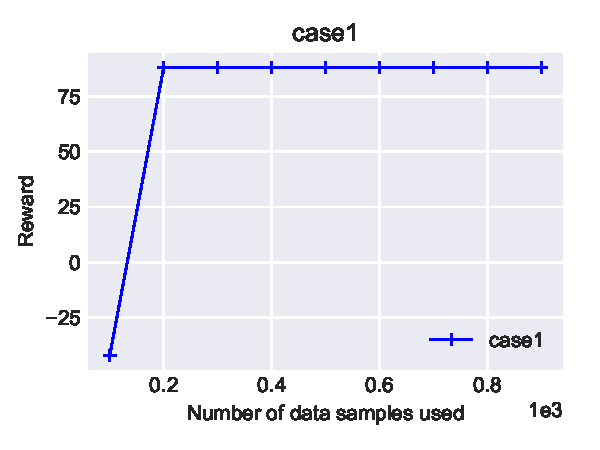
\includegraphics{pic/case1/case1.pdf}
    \caption{累计奖赏值曲线}
    \label{6-2}
\end{figure}
可以看出,在两次采样和训练周期后,模型的奖赏值就收敛到了一个稳定的全局最优值。同时我们将Q-leanring的查找表也做了可视化分析,进一步确认智能体学到一个实际有效的策略。首先我们选择了三个点$(3, 0), (2, 0), (0, 0), (3,3)$的对应4个行为的状态行为函数的变化过程,并进行分别进行比较。在起始点$(3,0)$时,显然向左或向右走优于其他行为,因为该情况下只有向左或向上为合法动作。在$(2, 0$点时,四个动作都为合法动作,但明显向左或向上走更接近目标,因此此时采取向左或向右也应该具有更高的Q值。同理在在$(0, 0)$和$(3,3)$点时,前者向上和后者向左走分别为最优策略。\par

\begin{figure}[h]
	\subfigure[]{
		\label{00}
		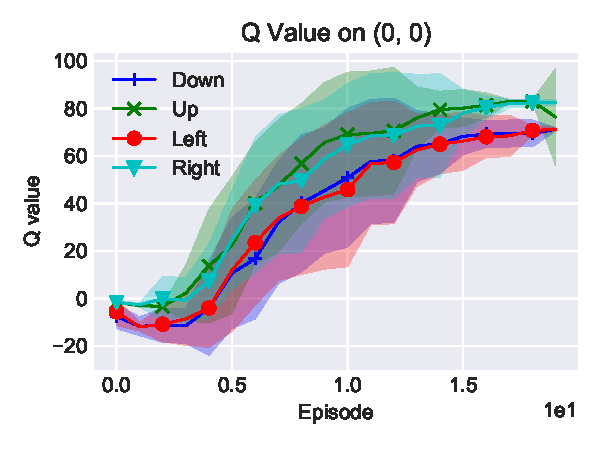
\includegraphics[width=7.3cm]{pic/case1/00.pdf}}
	\subfigure[]{
		\label{20}
		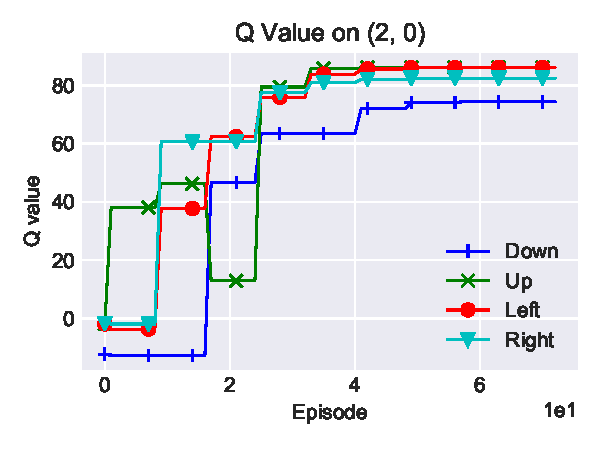
\includegraphics[width=7.3cm]{pic/case1/20.pdf}}
	\caption{Q 值在点(0,0)和点(2,0)的变化曲线}
	\label{fig1}
\end{figure}

\begin{figure}[h]
	\subfigure[]{
		\label{00}
		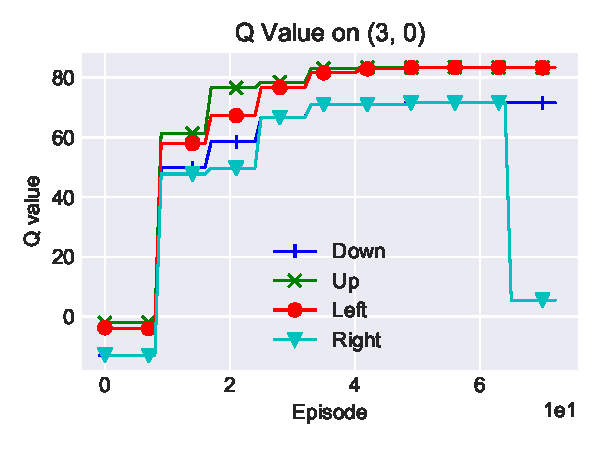
\includegraphics[width=7.3cm]{pic/case1/30.pdf}}
	\subfigure[]{
		\label{20}
		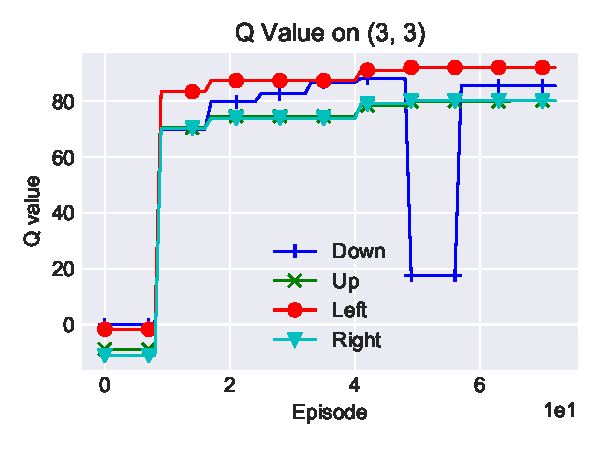
\includegraphics[width=7.3cm]{pic/case1/33.pdf}}
	\caption{Q 值在点(3,0)和点(3,3)的变化曲线}
	\label{fig2}
\end{figure}

\subsection{场景2}
在场景2中,我们的地图环境和场景1相同,但加入了额外的转弯损失,当智能体选择左转或掉头时,会得到额外的20的乘法。对于智能体,采用相同的$\epsilon-Greedy$策略和相同的参数设置。因为我们需要加入转弯的信息用于智能体决策,所以对应的 Q-leanring 的查找表的大小按照 xx 节的定义为$4^2 \cdot N\cdot M$,即加入额外的一维记录上一时刻的车辆方向的状态,使得智能体能够获得关于是否触发左转动作的信息。由于 Q-learning 的查找表规模变大,因此在实验中,我们将迭代次数增加为50次。图 xx 展示了智能体在测试时的累计奖赏,可以看到模型稳定的收敛在了最优策略上。
\begin{figure}
    \centering
    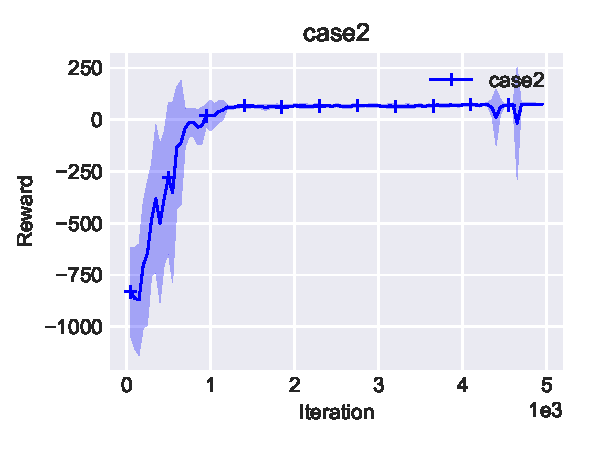
\includegraphics{pic/case2/case1.pdf}
    \caption{累计奖赏值曲线}
    \label{case2-1}
\end{figure}
类似场景1,现在我们对部分状态的状态动作价值函数可视化,我们展示在同一位置坐标下,不同的动作的 Q 函数在上一个时刻的4个动作上的均值,显然,在该场景下,右转和直行应当比左转具有更高的 Q 值。在该场景下,仅存在唯一的最优策略为从起点(0,0)出发,向上到达(0,3)后,右转到达终点(3,3),这样避免了左转带来的额外消耗。所以在(0,0)点时,不同于场景1的Up 和 Right具有相同的 Q 值,在该场景下 Up 显著高于 Right,如图 xx 所示。然后我们检查当智能体处在(3,0)且上一时刻方向为向右时的Q值大小,即当智能体处在只能选择左转才能以最短路径到达时,检测是否会因为额外转弯的惩罚丢失掉最优策略,实验结果最终展示为智能体优先选择了路径最短的点,而不是避免左转,如图 xx 所示。最后我们随机选择(0,2)(0,3)两个点可视化其 Q 值,如图 xxx 所示。
\begin{figure}[h]
	\subfigure[]{
		\label{00}
		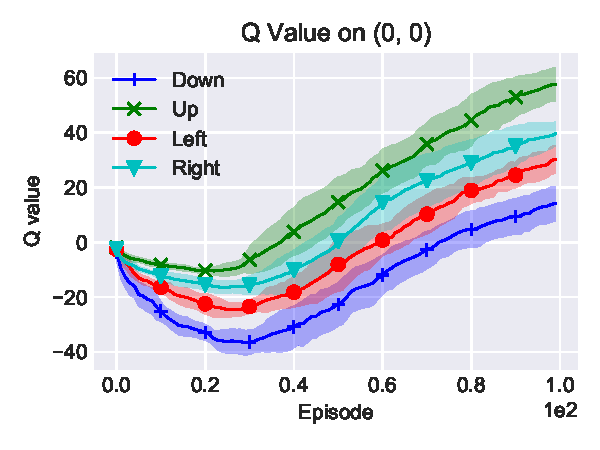
\includegraphics[width=7.3cm]{pic/case2/00.pdf}}
	\subfigure[]{
		\label{20}
		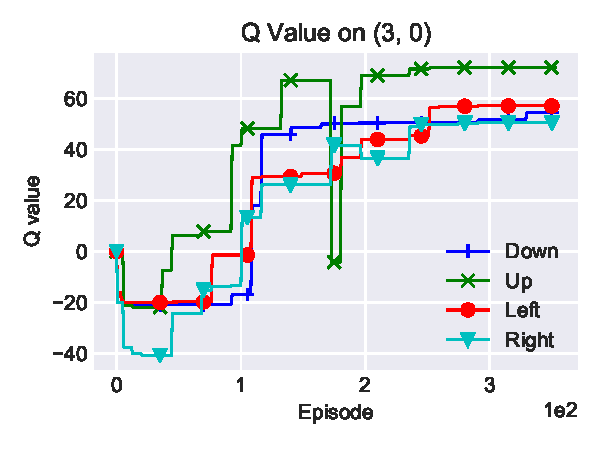
\includegraphics[width=7.3cm]{pic/case2/30.pdf}}
	\caption{Q 值在点(0,0),(3,0)的变化曲线}
	\label{fig1}
\end{figure}

\begin{figure}[h]
	\subfigure[]{
		\label{00}
		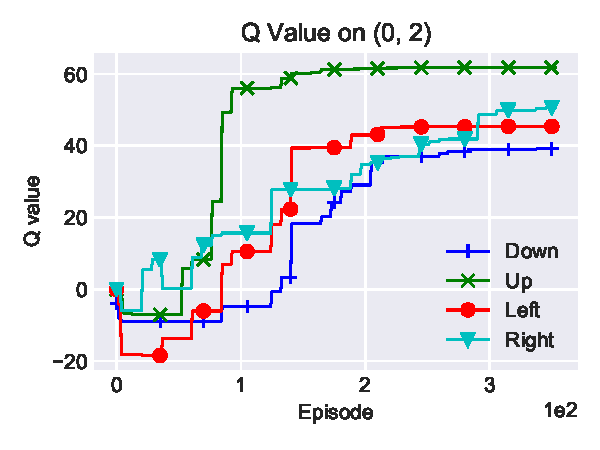
\includegraphics[width=7.3cm]{pic/case2/02.pdf}}
	\subfigure[]{
		\label{20}
		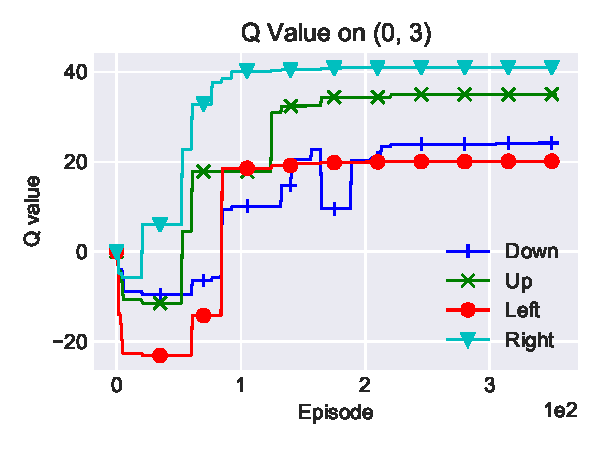
\includegraphics[width=7.3cm]{pic/case2/03.pdf}}
	\caption{Q 值在点(0,3)和点(0,2)的变化曲线}
	\label{fig2}
\end{figure}

\subsection{场景3}
在该场景中,我们对环境分别在(1,2)和(0,3)加入了充电桩,其他的设置与场景1保持相同,同时对奖赏函数的设计做了如下设置,如果在中途电量耗尽则返回额外的40的惩罚,如果到达充电桩,返回2的奖赏值。设置车辆在满电量时的行驶距离为3,单次移动消耗1单位电量。对于智能体,我们需要加入两个充电桩的位置以及当前的剩余电量到状态中,因此 Q 函数查找表的规模为$4\times 3 \cdot N^3 \cdot M^3$。首先我们给出智能体的测试环境下的累计奖赏值,可以看出智能体的策略收敛到了一个比较稳定的最优值。
另外由于该问题的特殊性,我们对最优路径做了可视化 tobe done!!!!!!!!!!1


\begin{figure}[h]
	\subfigure[]{
		\label{00}
		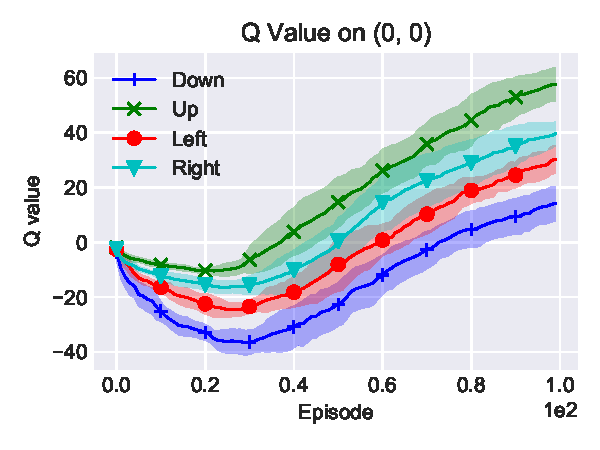
\includegraphics[width=7.3cm]{pic/case2/00.pdf}}
	\subfigure[]{
		\label{20}
		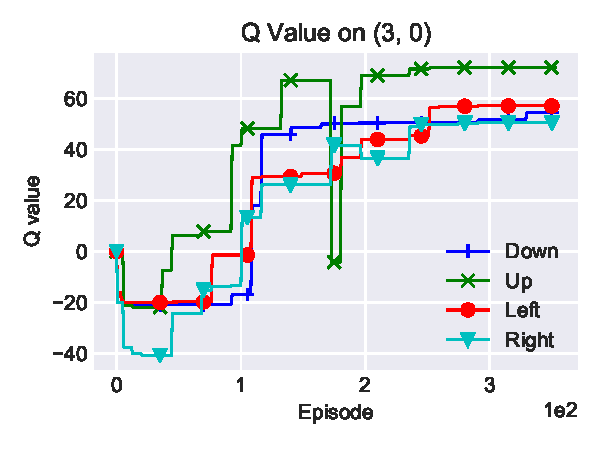
\includegraphics[width=7.3cm]{pic/case2/30.pdf}}
	\caption{Q 值在点(0,0),(3,0)的变化曲线}
	\label{fig1}
\end{figure}

\begin{figure}[h]
	\subfigure[]{
		\label{00}
		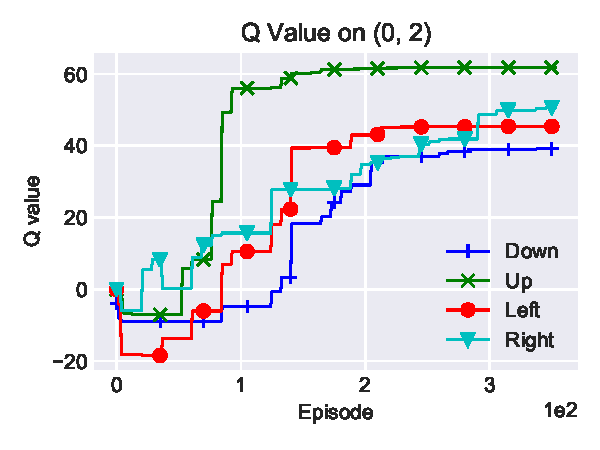
\includegraphics[width=7.3cm]{pic/case2/02.pdf}}
	\subfigure[]{
		\label{20}
		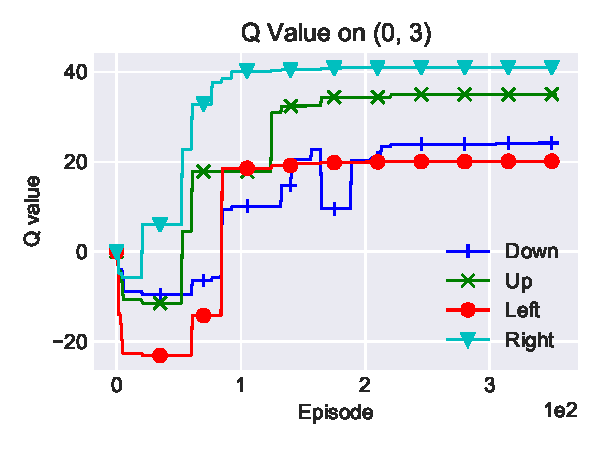
\includegraphics[width=7.3cm]{pic/case2/03.pdf}}
	\caption{Q 值在点(0,3)和点(0,2)的变化曲线}
	\label{fig2}
\end{figure}

% \subsection{场景4}
\subsection{本章小结}
在本章,我们给出了代码的实现细节,实验的参数设置和实验结果。通过实验结果的展示,验证了我们的算法实际学习到了合理的策略,表现出了其效果和有效性。同样在调参过程中我们发现了相应的问题,使得以后的相关研究可以进行借鉴参考。
\end{document}